\documentclass{beamer}

%%%% Packages
\usepackage{amsmath, amsthm, amssymb}
\usepackage[english]{babel}
\usepackage{array}              % for >{} in table column
% specification
\usepackage{color}              % for color definition
\usepackage{colortbl}
\usepackage{graphicx}
\usepackage{multirow}           % for multirow
\usepackage{multicol}           % for multiple columns
\usepackage{tabularx}           % for centering in table
\usepackage{tikz}               % for drawing diagrams
\usetikzlibrary{arrows}

%%%% Macros and Definitions
\definecolor{firebrick4}{RGB}{139,026,026}
\definecolor{gray57}{RGB}{145,145,145}
\definecolor{gray71}{RGB}{181,181,181}
\definecolor{gray84}{RGB}{212,212,212}
\definecolor{lightcyan4}{RGB}{122,139,139}
\definecolor{dodgerblue4}{RGB}{16,78,139}
\definecolor{dodgerblue3}{RGB}{24,116,205}

\newcommand{\indentpar}[1]{{\setlength{\parindent}{1cm} #1}}

%%%% Presentation Setup
\mode<presentation>
    {
      \usetheme{Ilmenau}
      \usecolortheme{beaver}
      \usefonttheme[onlylarge]{structuresmallcapsserif}
    }
    \setbeamercolor{title}{fg=dodgerblue4}
    \setbeamercolor{frametitle}{fg=dodgerblue4}
    \setbeamercolor*{palette secondary}{fg=dodgerblue4,bg=gray84}
    \setbeamercolor*{palette tertiary}{fg=white,bg=dodgerblue4}
    \setbeamercolor*{item}{fg=dodgerblue4}

    \setbeamerfont{author}{size=\scriptsize}
    \setbeamerfont{institute}{size=\scriptsize}
    \setbeamerfont{date}{size=\tiny}
    \setbeamerfont{normal text}{size=\scriptsize}

    \beamertemplatenavigationsymbolsempty

    %%%% Title
    \title[Report 2014]{PhD Report -- Spring 2014}
    \author[Sidorenko]{Wladimir Sidorenko\\ \texttt{uladzimir.sidarenka{@}uni-potsdam.de}}
    \institute[Uni Potsdam]{University of Potsdam}
    \date{\today}

    \pgfdeclareimage[interpolate=true,height=2.5cm]{logo}{img/uni_potsdam_logo.png}
    \titlegraphic{\pgfuseimage{logo}}

    %%%% Document
    \begin{document}
    %%%%%%%%%%%%%%%%%%%%%%%%%%%%%%%%%%%%%%%%%%%%%%%%%%%%%%%%%%%%%%%%%%
    %%% Title Page
    \begin{frame}{}
      \titlepage
    \end{frame}

    %%%%%%%%%%%%%%%%%%%%%%%%%%%%%%%%%%%%%%%%%%%%%%%%%%%%%%%%%%%%%%%%%%
    %%% Table of Contents
    \begin{frame}{Table of Contents}
      \tableofcontents
    \end{frame}

    %%%%%%%%%%%%%%%%%%%%%%%%%%%%%%%%%%%%%%%%%%%%%%%%%%%%%%%%%%%%%%%%%%
    %%% Sentiment Corpus
    \section{Sentiment Corpus}
    \subsection{Composition Criteria}
    \begin{frame}{\insertsubsection}
      For developing and testing our sentiment analysis system, we
      have created a corpus of 3996 Twitter messages.  This corpus
      consists of four major topic parts (two political and two
      non-political ones) each of which was sampled using three
      disjoint selection criteria.
    \end{frame}

    \begin{frame}{\insertsubsection}
      The covered topics are:
      \begin{enumerate}
      \item Political:
        \begin{itemize}
        \item Tweets containing political terms {\tiny(March 27 --
          May 25, 2013)};
        \item Tweets pertaining to the federal election 2013
          {\tiny(June 15 -- September 30, 2013)};
        \end{itemize}

      \item Non-political:
        \begin{itemize}
        \item General tweets with no particular topic {\tiny(March
          31 -- April 30, 2013)};
        \item Tweets pertaining to the pope election 2013
          {\tiny(March 13 -- March 14, 2013)}.
        \end{itemize}
      \end{enumerate}
    \end{frame}

    \begin{frame}{\insertsubsection}
      The selection criteria for each of the topics are:
      \begin{enumerate}
      \item Presence of polar terms (SentiWS \cite{Remus-10});
      \item Presence of smileys and exclamation marks;
      \item Others.
      \end{enumerate}
      For each of the above criteria, we sampled 333 messages for each
      topic.  All messages were sampled disjointly so that tweets
      which fell into one of the preceding categories were excluded
      from the next ones.
    \end{frame}

    \subsection{Annotation Scheme}
    \begin{frame}{\insertsubsection}
      \textbf{Emo-expressions} (\textit{expressive subjective
        elements} \cite{Wiebe-05}) - lexical items with polar
      evaluative sense, e.g. \textit{gut, schrecklich, kritisieren,
        zum Besten halten etc.};

      \textbf{Diminishers} (\textit{down-turners} \cite{Taboada-11}) -
      words or phrases which decrease the intensity of an
      emo-expression term, e.g. \textit{weniger, bisschen, kaum etc.}

      \textbf{Intensifiers} - lexical elements which strengthen the
      polar evaluative sense of an emo-expression, e.g. \textit{recht,
        super, au\ss{}erordentlich etc.}

      \textbf{Negations} - language elements which reverse the
      polarity of subjective meaning expressed by an ESE,
      e.g. \textit{nicht, kein, etc.}
    \end{frame}

    \begin{frame}{\insertsubsection}
      \textbf{Sentiment} - minimal complete coherent syntactic or
      discourse-level unit that expresses a polar evaluative opinion
      of a person or organization about some particular subject,
      topic, or event, e.g. \textit{Ich hasse diese Reform},
      \textit{ein ausgezeichneter Film}, \textit{Meine Mutter ruft
        mich heulend an.  Man hat einen Argentinier zum Papst
        gew\"ahlt.};

      \textbf{Source} - the immediate originator of a polar evaluative
      opinion who either directly expresses her opinion or whose
      opinion is being cited;

      \textbf{Target} - subject or event which is being evaluated in a
      sentiment.
    \end{frame}

    \begin{frame}{\insertsubsection}
      \begin{example}
        \begin{math}
        [[\text{Ich}]_{\text{\bfseries source}}
          [\text{hasse}]_{\text{\bfseries emo-expression}}
          [\text{Merkel}]_{\text{\bfseries target}}]_{\text{\bfseries sentiment}}\text{.}
        \end{math}
      \end{example}
    \end{frame}

    \subsection{Preliminary Statistics}
    \begin{frame}{\insertsubsection}
      \begin{table}
        \caption{\scriptsize Distribution of emotional expressions
          across topics and selection criteria in corpus.}  \centering
        \begin{tabular}{p{0.25\textwidth}*{4}{>{\centering\arraybackslash}p{0.15\textwidth}}}
          \hline\noalign{\smallskip}
          \multirow{2}{*}{Selection Criterion} & %
          \multicolumn{2}{c}{\texttt{Politics}} & %
          \multicolumn{2}{c}{\texttt{Non-politics}}\\
          & General Politics & Federal Election & General Discussions & Pope Election\\
          \noalign{\smallskip} \hline
          Polar Terms & 225 & 199 & 270 & 163\\
          Emoticons & 426 & 415 & 457 & 364\\
          Other & 76 & 75 & 82 & 54\\
          \noalign{\smallskip} \hline
        \end{tabular}
      \end{table}
    \end{frame}

    \begin{frame}{\insertsubsection}
      \begin{table}
        \caption{\scriptsize Distribution of sentiments across topics
          and selection criteria in corpus.}  \centering
        \begin{tabular}{p{0.25\textwidth}*{4}{>{\centering\arraybackslash}p{0.15\textwidth}}}
          \hline\noalign{\smallskip}
          \multirow{2}{*}{Selection Criterion} & %
          \multicolumn{2}{c}{\texttt{Politics}} & %
          \multicolumn{2}{c}{\texttt{Non-politics}}\\
          & General Politics & Federal Election & General Discussions & Pope Election\\
          \noalign{\smallskip} \hline
          Polar Terms & 90 & 105 & 79 & 83\\
          Emoticons & 68 & 71 & 35 & 50\\
          Other & 54 & 46 & 17 & 30\\
          \noalign{\smallskip} \hline
        \end{tabular}
      \end{table}
    \end{frame}

    %%%%%%%%%%%%%%%%%%%%%%%%%%%%%%%%%%%%%%%%%%%%%%%%%%%%%%%%%%%%%%%%%%
    %%% Sentiment Analysis
    \section{Sentiment Analysis}
    \subsection{Classifiers}
    \begin{frame}{\insertsubsection}
      \begin{table}
        \caption{\scriptsize Classification results for automatic
          sentiment analysis (token-based).}
        \centering
        \begin{tabular}{p{0.25\textwidth}*{4}{>{\centering\arraybackslash}p{0.15\textwidth}}}
          \hline\noalign{\smallskip}
          ML-System& Sentiment & Source & Target & Other\\\hline
          MLN & na & na & na & na\\
          SVM & 3.4 & 10.7 & 0 & 94.5\\
          Bayes Net & 15.7 & 9.4 & 5.8 & 89\\
          NB & 15.9 & 7.5 & 8.9 & 78.4\\
          Multinomial NB & 17.5 & 9.8 & 11 & 85.6\\
          CRF & 16.53 & 17.65 & 7.89 & 94.47\\
          \noalign{\smallskip} \hline
        \end{tabular}
      \end{table}
    \end{frame}

    \subsection{CRF}
    \begin{frame}{\insertsubsection}
      Features:
      \begin{multicols}{2}
        \begin{itemize}
        \item Formal:
          \begin{itemize}
            \tiny
          \item Initial three characters of word form;
          \item Final three characters of word form;
          \item Character class of word (title, upper, lower,
            alphabetic mixed, alnum, digit, punct, mixed);
          \end{itemize}
        \item Morphological:
          \begin{itemize}
            \tiny
          \item Case;
          \item Gender;
          \item Degree of Comparison;
          \item Mood;
          \item Tense;
          \item Person;
          \end{itemize}
        \item Lexical:
          \begin{itemize}
            \tiny
          \item Word Form;
          \item Polarity Score (SentiWS* \cite{Remus-10} and
            GermanPolarityClues \cite{Waltinger-10});
          \item Class of modal verb (lexical or true modal);
          \end{itemize}
        \item Syntactical:
          \begin{itemize}
            \tiny
            \item Dependency relation of preceding and current word;
            \item Dependency relation of current word;
            \item Dependency relation of current and next word;
            \item Lemma of parent;
            \item PoS-Tag of grandmother;
            \item Form of grandmother;
            \item Polarity class of grandmother;
            \item Child Lemma + Dependency Relation;
            \item Child Lemma + Dependency Relation + Lemma;
            \item Child PoS-Tag + Dependency Relation + PoS-Tag;
            \item Cummulative polarity class for children (polarity
              class of the sum of children's scores);
          \end{itemize}
        \end{itemize}
      \end{multicols}
    \end{frame}

    \subsection{Evaluation}
    \begin{frame}{\insertsubsection}
      Evaluation schemes:
      \begin{itemize}
        \scriptsize
        \item<1-> Binary Overlap \cite{Breck-07}:\\
          \begin{math}\textstyle
            \text{Precision} = \frac{|\left\{p| p \in P \wedge \exists
              c \in C \text{ s.t. } f(c,p)\right\}|}{|P|}\text{; }
            \text{Recall} = \frac{|\left\{c| c \in C \wedge \exists p
              \in P \text{ s.t. } f(c,p)\right\}|}{|C|};
          \end{math}\\
          where $C$ is the set of correct spans, $P$ is the set of
          predicted spans, and $f(c, p)$ is a function which yields
          ``true'' if the spans overlap and ``false'' otherwise;
        \item<2-> Proportional Overlap \cite{Johansson-10}:\\
          \begin{math}\textstyle
            \text{Precision} = \frac{\text{Score}(C, P)}{|P|}\text{;
            }\text{Recall} = \frac{\text{Score}(P, C)}{|C|};
          \end{math}\\
          where $\text{Score}(S, S') = \sum_{s \in S}\sum_{s' \in
            S'}f(s, s')$ and $f(s, s') = \frac{|s \cap s'|}{|s'|}$;
        \item<3-> Exact Match \cite{Breck-07}:\\ the same as
          binary overlap except that $f(c, p)$ yields ``true'' iff the
          compared spans completely agree on their boundaries.
      \end{itemize}
    \end{frame}

    \begin{frame}{\insertsubsection}
      \begin{table}
        \tiny
        \caption{\scriptsize Classification results for automatic
          sentiment analysis (binary overlap). \visible<2>{\alert{Sentiment is ESE}}}  \centering
        \begin{tabular}{p{0.25\textwidth}*{3}{>{\centering\arraybackslash}p{0.15\textwidth}}}
          \hline\noalign{\smallskip}
          Classification Element & Precision & Recall & F-Measure\\\hline
          \multicolumn{4}{c}{\cellcolor{lightcyan4}Training Set}\\
          \alt<1>{
            Sentiment & 99.23 & 86.27 & 92.29\\
            Source & 91.56 & 75.55 & 82.78\\
            Target & 95.99 & 75.69 & 84.64\\
          }{
            Sentiment & 94.38 & 81.43 & 87.43\\
            Source & 92.31 & 48.54 & 63.62\\
            Target & 96.95 & 56.83 & 71.66\\
          }
          \hline\multicolumn{4}{c}{\cellcolor{lightcyan4}Test Set}\\
          \alt<1>{
            Sentiment & 25 & 16.04 & 19.55\\
            Source & 47.06 & 25 & 32.65\\
            Target & 31.51 & 18.11 & 23\\
          }{
            Sentiment & 76.54 & 68.5 & 72.29\\
            Source & 25 & 18.75 & 21.43\\
            Target & 15.46 & 11.81 & 13.39\\
          }
          \noalign{\smallskip} \hline
        \end{tabular}
      \end{table}
    \end{frame}

    \begin{frame}{\insertsubsection}
      \begin{table}
        \tiny
        \caption{\scriptsize Classification results for automatic
          sentiment analysis (proportional overlap). \visible<2>{\alert{Sentiment is ESE}}}\centering
        \begin{tabular}{p{0.25\textwidth}*{3}{>{\centering\arraybackslash}p{0.15\textwidth}}}
          \hline\noalign{\smallskip}
          Classification Element & Precision & Recall & F-Measure\\\hline
          \multicolumn{4}{c}{\cellcolor{lightcyan4}Training Set}\\
          \alt<1>{
            Sentiment & 97.62 & 84.94 & 90.84\\
            Source & 90.4 & 73.71 & 81.21\\
            Target & 93.55 & 74.02 & 82.65\\
          }{
            Sentiment & 93.62 & 80.5 & 86.57\\
            Source & 92.07 & 48.26 & 63.33\\
            Target & 94.39 & 55.58 & 69.96\\
          }
          \hline\multicolumn{4}{c}{\cellcolor{lightcyan4}Test Set}\\
          \alt<1>{
            Sentiment & 21.31 & 14.53 & 17.28\\
            Source & 40 & 25 & 30.77\\
            Target & 26.06 & 13.75 & 18\\
          }{
            Sentiment & 74.38 & 67.27 & 70.65\\
            Source & 22.22 & 18.75 & 20.34\\
            Target & 12.16 & 10.56 & 11.3\\
          }
          \noalign{\smallskip} \hline
        \end{tabular}
      \end{table}
    \end{frame}


    \begin{frame}{\insertsubsection}
      \begin{table}
        \tiny
        \caption{\scriptsize Classification results for automatic
          sentiment analysis (exact match). \visible<2>{\alert{Sentiment is ESE}}}\centering
        \begin{tabular}{p{0.25\textwidth}*{3}{>{\centering\arraybackslash}p{0.15\textwidth}}}
          \hline\noalign{\smallskip}
          Classification Element & Precision & Recall & F-Measure\\\hline
          \multicolumn{4}{c}{\cellcolor{lightcyan4}Training Set}\\
          \alt<1>{
            Sentiment & 87.37 & 72.7 & 79.36\\
            Source & 88.24 & 71.17 & 78.79\\
            Target & 85.54 & 66.44 & 74.79\\
          }{
            Sentiment & 90.9 & 78.39 & 84.18\\
            Source & 89.51 & 46.72 & 61.39\\
            Target & 80.08 & 45.6 & 58.11\\
          }
          \hline\multicolumn{4}{c}{\cellcolor{lightcyan4}Test Set}\\
          \alt<1>{
            Sentiment & 13.95 & 9.09 & 11.01\\
            Source & 40 & 25 & 30.77\\
            Target & 14.67 & 8.66 & 10.89\\
          }{
            Sentiment & 70.84 & 63.21 & 66.81\\
            Source & 20.83 & 15.62 & 17.86 \\
            Target & 8.25 & 6.3 & 7.14\\
          }
          \noalign{\smallskip} \hline
        \end{tabular}
      \end{table}
    \end{frame}

    \begin{frame}{Learning Curve}
      \begin{figure}
        \centering
        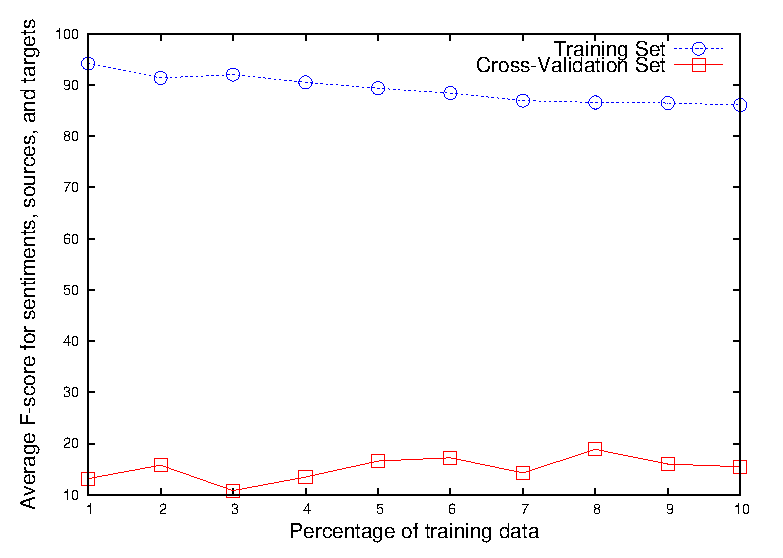
\includegraphics[width = 0.9\textwidth,height=170px]{img/lrn_curve.eps}
      \end{figure}
    \end{frame}

    \begin{frame}{Problems and Open Questions}
      \begin{itemize}
        \item Bad overfitting;
        \item Polarity detection;
        \item Flat tagging scheme;
        \item Relation linking.
      \end{itemize}
    \end{frame}

    \begin{frame}{Preliminary Conclusions and Perspectives}
      Conclusions:
      \begin{itemize}
        \item Preprocessing matters (w/25.067 vs. wo/18.277);
        \item Quality of polarity dictionaries is important (sentiws/25.067 vs. gpc/23.903);
      \end{itemize}

      Perspectives:
      \begin{itemize}
        \item Different classifiers (higher order CRFs, structural SVMs, etc.);
        \item Experiments with polarity dictionaries and ontologies;
      \end{itemize}
    \end{frame}

    %%%%%%%%%%%%%%%%%%%%%%%%%%%%%%%%%%%%%%%%%%%%%%%%%%%%%%%%%%%%%%%%%%
    %%% Discourse Segmentation
    \section{Discourse Analysis}
    \subsection{Connectives}
    \begin{frame}{\insertsubsection}
      \tiny
      \begin{table}
        \caption{\scriptsize Approximate distribution of discourse
          connectives in corpus.}  \centering
        \begin{tabular}{p{0.25\textwidth}*{2}{>{\centering\arraybackslash}p{0.3\textwidth}}}
          \hline\noalign{\smallskip}
          \multirow{2}{*}{Top-10 Connectives} & %
          \multicolumn{2}{c}{\texttt{\# of tweets}}\\
          & Non-Answers & Answers\\
          \noalign{\smallskip} \hline
          und & 2,787,798 & 769,301\\
          f\"ur & 1,734,911 & 267,975\\
          auch & 596,142 & 599,445\\
          wie & 559,449 & 287,471\\
          aber & 366,489 & 397,896\\
          oder & 318,181 & 172,969\\
          dass & 301,296 & 131,624\\
          ja & 290,461 & 414,543\\
          dann & 288,707 & 241,499\\
          da & 269,446 & 228,490\\
          \multicolumn{3}{c}{}\\
          Percent of tweets with connectives & 37\% & 49\%\\
          \noalign{\smallskip} \hline
        \end{tabular}
      \end{table}
    \end{frame}

    \begin{frame}{Discourse Relations}
      \begin{table}
        \tiny
        \caption{\scriptsize Approximate distribution of discourse relations in corpus.}  \centering
        \begin{tabular}{p{0.25\textwidth}*{2}{>{\centering\arraybackslash}p{0.3\textwidth}}}
          \hline\noalign{\smallskip}
          \multirow{2}{*}{Top-10 Discourse Relations} & %
          \multicolumn{2}{c}{\texttt{\# of tweets}}\\
          & Non-Answers & Answers\\
          \noalign{\smallskip} \hline
          Elaboration* & 4,620,913 & 1,917,685\\
          Sequence & 1,397,751 & 735,492\\
          Concession* & 106,0244 & 894,494\\
          Circumstance & 928,997 & 400,505\\
          Contrast* & 918,498 & 777,630\\
          Cause & 895,181 & 624,868 \\
          Anthithese* & 471,187 & 518,792\\
          Joint & 401,916 & 285,196\\
          Substitution & 104,074 & 25,067\\
          Unconditional & 99,904 & 41,589\\
          \noalign{\smallskip} \hline
        \end{tabular}
      \end{table}
    \end{frame}

    \subsection{Discourse Segmenter}
    \begin{frame}{\insertsubsection}
      \scriptsize
      ! @DJVBB Wulff hat nicht get\"auscht, sondern wegen der Mehrfachbelastung als junger Familienvater den \"Uberblick \"uber die Geldquellen verloren.\\[0.5cm]
      (\textbf{"sondern"}\\
      \indentpar{\scriptsize(\textbf{intern}: wegen/APPR der/ART Mehrfachbelastung/NN als/KOKOM junger/ADJA Familienvater/NN den/ART \"Uberblick/NN \"uber/APPR die/ART Geldquellen/NN verloren/VVFIN)\\
      (\textbf{extern}: Wulff/NE hat/VAFIN nicht/PTKNEG get\"auscht/VVPP ,/\$,))}\\[0.5cm]
      (\textbf{"wegen"}\\
      \indentpar{\scriptsize(\textbf{intern}: der/ART Mehrfachbelastung/NN)}\\
      \indentpar{\scriptsize(\textbf{extern}: Wulff/NE hat/VAFIN nicht/PTKNEG get\"auscht/VVPP ,/\$, sondern/KON wegen/APPR der/ART Mehrfachbelastung/NN als/KOKOM junger/ADJA Familienvater/NN den/ART \"Uberblick/NN \"ber/APPR die/ART Geldquellen/NN verloren/VVFIN))}
   \end{frame}

    \begin{frame}{Perspectives and Future Work}
      \begin{itemize}
        \item Disambiguation of discourse connectives and relations;
        \item Analysis of discourse relations within and among the
          tweets (inter- and intra-tweet relations);
        \item Analysis of discourse relations and connectives in tweets expressing sentiments;
        \item Analysis of tweets expressing CONTRAST and ELEBORATION relations for sentiments.
      \end{itemize}
    \end{frame}

    \section*{Bibliography}
    \bibliography{bibliography}
    \bibliographystyle{plain}
    \end{document}
